%Document Class starts every LaTeX document.  In this case, we're declaring the document class to be a book.  Changing "oneside" to "twoside" changes where the page numbers and headers and such get placed.
\documentclass[12pt,oneside]{book}
\usepackage{thesis} % use thesis style file
\begin{document}


%===============================================================================
% TITLE PAGE / ABSTRACT / ACKNOWLEDGEMENTS
%===============================================================================
\frontmatter % this is the stuff that comes before the real text:

% The \include command inserts the external files into the final document:
%Here goes the title page:
\pagestyle{empty}
\begin{titlepage}
\begin{center}
\rule{5.75in}{1pt} \\
\vspace*{-0.125in}
{\large \doublespacing Wesleyan University} \hfill {\large \doublespacing The Honors College}
\rule[0.2in]{5.75in}{1pt} \\
\vspace*{0.8in}

% title
{\LARGE \singlespacing \bf 
  Using Vertical Structure to Infer \\
  the Dynamical Mass Hidden in \\
  the AU Mic Debris Disk
  } \\
\vspace*{0.05in}
\vspace*{0.10in}

{\large \vspace*{0.20in}  \singlespacing by \vspace*{.2in}
\\Cail Daley \\ Class of 2018\\}
\vspace*{0.25in}
\vspace*{0.8in}
{\large \singlespacing A thesis submitted to the\\ faculty of Wesleyan University\\ in partial fulfillment of the requirements for the \\ Degree of Bachelor of Arts\\ with Departmental Honors in Astronomy\\ \vspace*{-0.15in} }
\vspace*{.25in}
\rule{5.75in}{1pt} \\
\vspace*{-0.125in}
{\large \doublespacing Middletown, Connecticut \hfill April, 2018}
\rule[0.2in]{5.75in}{1pt} 
\end{center}
\end{titlepage}

% \pagestyle{empty}
% %\pagestyle{plain}

\mbox{}
\vspace{.75in}
\hrule

\vspace{2in}


%\begin{minipage}[c]{4in}
\begin{centering}
	\hspace{.25in} 
	\parbox{5in}{
		\noindent 
		\textit{We are just an advanced breed of monkeys on a minor planet of a very average star. But we can understand the Universe. That makes us something very special.}
		\vspace{3pt}

		\begin{flushright}
			{\sc {--Stephen Hawking}}\\
		%	{\textit{The Hitchhiker's Guide to the Galaxy}}
		\end{flushright}
	}
\end{centering}
\vspace{2.25in}
\hrule
\vfill



%\flushleft















\textwidth 5.750in \textheight=8.50in \headheight 0.0625in \topmargin 0.0in % book strict

% \chapter{Acknowledgements}

I would like to thank Meredith Hughes for being an amazing mentor through the process of teaching me to do advanced research, all the way from the crash course in radio astronomy at the beginning of my Junior year through this thesis. I'm blessed to have worked with such a dedicated advisor who cares so much about the learning process for each and every student. Going to Hawaii to observe at the SMA and Seattle for AAS were unforgettable experiences that not many undergraduates have, but those are really just cherries on top of the incredible sundae of knowledge, experience, and wisdom that you've passed on to me. 

Thanks to Seth Redfield for selling me on the astronomy program here at Wesleyan and getting me involved with the 24$''$ observing program. I may never live down getting flung from my chair as the monkey in an angular momentum demonstration he put me up to, but at least I'm better at ultimate frisbee. 

Thanks to Kevin Flaherty, for helping me out with everything from cluster computing to statistical tests, and to Roy Kilgard, for the endless patience in helping me with computer issues and always being fun to stop by and talk to. Thanks to Angelo Ricarte for writing the foundation of the modeling code that I used in this thesis. 

To Mom and Dad, thanks for giving me multiplication problems before bed to help me fall asleep, even if you didn't always know the correct answer. I wouldn't be who I am today without your love and guidance. Mira, you're the best sister a little bro could ask for. 

To the basement crew, thanks for endless entertainment in times of drastic procrastination, playing darts, and letting me fly the baby drone around the library when that was our workspace without going crazy (RIP baby drone. Both a sorry and a damn you to the Fisk Telescope for breaking the last propellor). 

\titlespacing*{\chapter}{0pt}{*2}{*3}



%===============================================================================
% TABLE OF CONTENTS
%===============================================================================

% LaTeX creates a table of contents for you automatically, 
% but you may have to compile the document twice before it shows up properly:
% \tableofcontents % \pagestyle{empty}

%You can also put in the following, if you wish:
%\listoffigures
%\listoftables \pagestyle{empty}


%===============================================================================
% CHAPTERS
%===============================================================================
\mainmatter % Now we start the real part of the document:
% \chapter{Observations}
\label{chap:obs}


\chapter{Observations}
AU Mic was observed  with ALMA on three dates: 26 March 2014, 18 August 2014, and 24 June 2015. 
All observations were configured with four spectral windows, and employed ALMA's 12m antennas and Band 7 receivers. 
Within each observation AU Mic was observed in seven-minute segments.\footnote{Extraneous?}
One spectral window was centered around the CO $J = (2-1)$ transition at a frequency of 230.538001 GHz, with a total bandwidth of 1.875 GHz and a channel spacing of 488 kHz.
The remaining three spectral windows were configured to detect continuum emission with central frequencies of 228.5, 213.5, and 216.0 GHz, total bandwidths of 2 GHz, and channel spacings of 15.6 MHz. 

\begin{table}	
  \centering
	\caption{Observation Information}
  \label{tab:observations}
  \begin{tabular}{lrrrr}
    \toprule
    & 26 March 2014 & 18 August 2014 & 24 June 2015 \\
    \cmidrule(lr){2-4}
    Antennas: & 32 & 35 & 37 \\
    Baselines (m): & 14--437 & 20--1268 & 30--1431 \\
    On-source time (min): & 35 & 35 & 33 \\
    Flux calibrator: & Titan & J2056-472 & Titan \\
    Bandpass calibrator: & J1924-2914 & J2056-4714 & J1924-2914 \\
    Phase calibrator: & J2101-2933 & J2101-2933 & J2056-3208  \\
    pwv (mm): & 0.6 & 1.6 & 0.7 \\
    \bottomrule
  \end{tabular}
\end{table}

Information regarding the three observation dates can be found in Table \ref{tab:observations}. 
The short-baseline March observation provides information about AU Mic's disk on large spatial scales; in contrast, the subsequent long-baseline August observation was intended to trace the small-scale structure of the disk. 
The quality of the gain transfer for the August observation was tested using observations of the quasar J2057-3734.
Due to subpar\footnote{too informal?} quality, the August data were supplemented with a second night of long-baseline observations in June 2015. 
The quasar J2101-2933 was used to assess the gain transfer quality.
During the last segment of the June observation (04:23:38-04:29:58 UT), the host star flared. While we initially fit and subtracted off the flare fluxes (see Table \ref{tab:flare fluxes}), it was ultimately decided that the data taken during the flare was too problematic to be included in our analysis.

\begin{table}	
  \centering
	\caption{Subtracted point-source fluxes}
  \label{tab:flare fluxes}
  \begin{tabular}{lr}
    \toprule
    Time (UTC) & Point-source Flux ($\mu$Jy) \\
    \midrule
    03:45:0--04:20:0 (no flare) & ($4.1 \pm 0.2)  \times 10^2$\\
  	4:23:38--4:24:00 & $(9.2 \pm 1.7) \times 10^2$ \\
  	4:24:00--4:25:00 & $(1.146 \pm 0.010) \times 10^4$ \\
  	4:25:00--4:26:00 & $(3.59 \pm 0.10) \times 10^3$ \\
  	4:26:00--4:27:00 & $(1.58 \pm 0.10) \times 10^3$ \\
  	4:27:00--4:28:00 & $(4.50 \pm 1.0) \times 10^2$ \\
  	4:28:00--4:29:00 & $(4.60 \pm 1.0) \times 10^2$ \\
  	4:29:00--4:29:58 & $(5.20 \pm 1.0) \times 10^2$\\
    \bottomrule
  \end{tabular}
\end{table}

Calibration, reduction, and imaging were carried out using the \texttt{CASA} and
\texttt{MIRIAD} software packages. Standard ALMA reduction scripts were applied
to the datasets: phase calibration was accomplished via water vapor radiometry
tables, and system temperature calibrations were performed to account for
variations in instrument and weather conditions. Flux and bandpass calibrations
were subsequently applied.


The authors travelled to the NRAO facility in Charlottesville, VA in October
2015 to further process the data in \texttt{CASA}. 
% in particular the trip was intended to allow on-site correction of the 24 June flare. 
% tasks used to reduce the data at the NRAO facility were all part of the CASA package. 
For each observation, an elliptical gaussian was fit with the task \texttt{imfit} to a small region around the star in the sky plane (for the June date, the flare data were excluded).
The equatorial coordinates of the the model gaussian centroid were then used to define the star position, which was uncertain due to AU Mic's high proper motion: each dataset was phase shifted using the task \texttt{fixvis} so that the pointing center of the data was the same as the fitted star position.

Imaging was performed via standard Fourier inversion using the \texttt{CASA} task \texttt{tclean}. 
Two weighting schemes were used: (i) natural weighting with no taper, to trace the small-scale disk structure and (ii) natural weighting with a \SI{200}{k\lambda} Gaussian taper applied to long baselines, to bring out the disk emission on larger spatial scales. 
Because the \texttt{CASA} task \texttt{tclean} preserves pointing center offsets when converting several visibility datasets into an image, it was necessary to combine the data into a single file before cleaning in order to account for the offset in phase center between datasets. 
This was done using the task \texttt{concat}, which combines datasets with pointing centers aligned so long as their pointing centers do not differ by a value greater than the parameter \texttt{dirtol} (set to a value of \SI{2}{''}).

\begin{table}
  \centering
  \caption{Imaging Parameters for AU Mic}
  \label{tab: imaging}
  \begin{tabular}{lrrr}
    \toprule
    Weighting Scheme & Beam Size (\si{''}) & Beam PA ($^\circ$) & RMS Noise (\si{\mu Jy}) \\
    \midrule
    Natural (no taper) & blank & blank & blank \\
    Natural (\SI{200}{k\lambda}) & blank & blank & blank \\
    \bottomrule
  \end{tabular}
\end{table}
% The peak flux of the model gaussian was also subtracted from the location of the star in the visibility domain so that only the disk remained.

% The 24 June dataset required additional reduction due to the flare. While for
% the other dates we were able to fit a single point source to account for the stellar
% component over the entire observation, the flare required that the dataset be
% split into one minute bins between 04:23:38 and 04:29:58 in order to account for
% the variable flux of the host star. For each of these bins, we used the task
% \texttt{uvmodelfit} to fit a point source to the long baseline visibilities,
% which we subsequently subtracted from each bin in the visibility domain.
% Subtracted point fluxes can be found in Table \ref{tab:flare fluxes}.

% The June date pointing center, defined by the centroid of the elliptical
% gaussian fit to the star, remained visibly offset from the disk; this
% could be explained if the flare referenced above were not symmetric with respect
% to the star. The offset was remedied by redefining the pointing center as
% follows. Because the star is known to be located at the center of the disk, we
% can use information provided by the brightness distribution of the disk to infer
% the star position. We do so by selecting the brightest pixel on each side of the
% disk from the clean component map (the \texttt{.model} file produced by
% \texttt{tclean}), and redefining the star/pointing center as the mean of the two
% pixel positions. This yields offsets of $(0.01'', -0.05'')$ for the March
% observation, $(0.01'', 0.00'')$ for the August observation, and $(0.00'',
% 0.09'')$ for the June observation. Given the good agreement between the
% calculated star position and the image center for the two non-flare dates (March
% and August), we conclude that the `pixel' method represents a viable way to
% accurately determine star position. We apply this correction and redefine the
% image center via \texttt{fixvis}. For consistency, we apply the phase shift to
% all three dates.

% Due to the high proper motion of AU Mic, the pointing centers of the three dates
% differ by a not-insignificant amount. When datasets with different pointing
% centers are cleaned together with \texttt{tclean}, the pointing center of the
% first dataset is taken as the new pointing center, and the data are combined in
% in the $uv$ plane with each subsequent dataset offset from the first as given by
% their relative pointing centers. In the case of AU Mic, this leads to an  image
% of the disk composed of three observations offset with respect to each other. To
% remedy this, we use the task \texttt{concat}, which combines datasets with their
% pointing centers aligned so long as the pointing centers do not differ by more
% than the value of \texttt{dirtol}. We set \texttt{dirtol} to $ 2''$, a value
% larger than  AU Mic's proper motion over ALMA's $\sim 1$ year observation
% baselines.

\chapter{Results}
AU Mic's disk is resolved in both the radial and vertical directions by the ALMA observations. The disk extends a distance of $\sim \SI{40}{au}$ on either side of the host star, although the NW side appears to reach slightly further radial extents than the SE side (\ref{fig: boccaletti}). However, we are not able to detect the PA offset described by \cite{boccaletti2015}

\begin{figure}
  \centering
  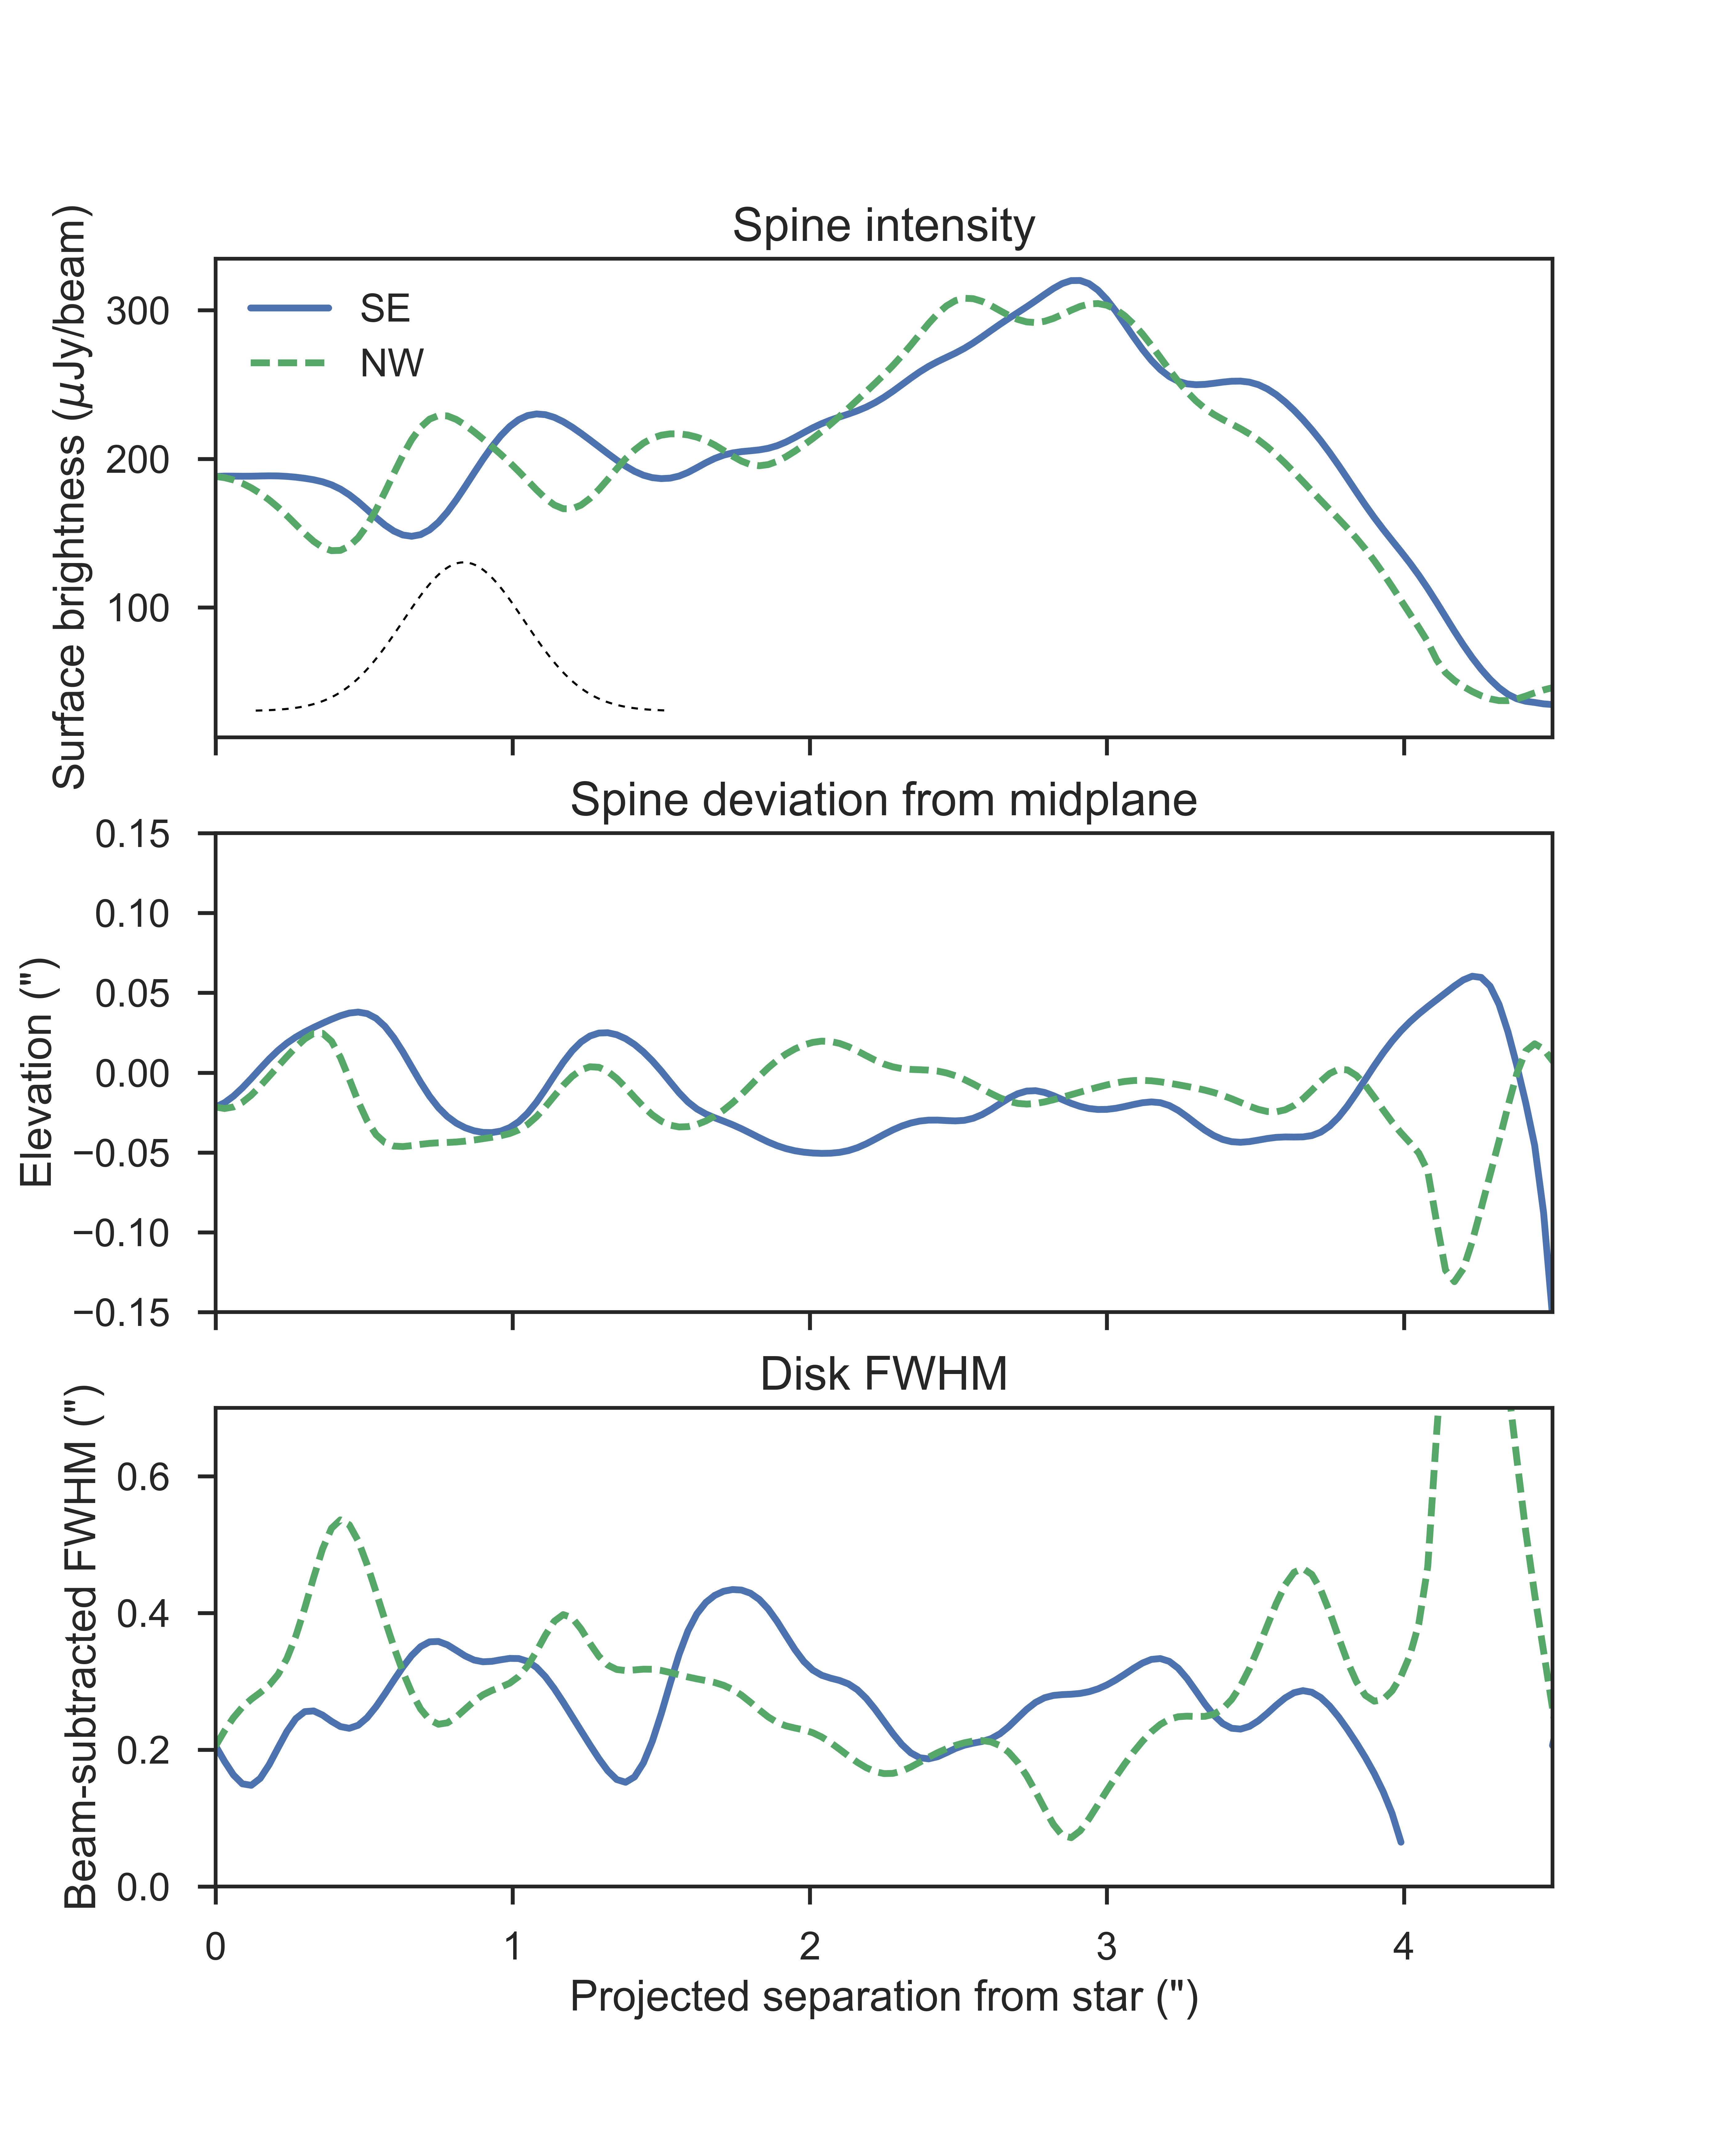
\includegraphics[width=.75\linewidth]{figures/3_boccaletti_plots}
  \caption{
  Image-domain analysis of AU Mic's radial structure. 
  At each radial location, a Gaussian was fit to the surface brightness profile created by taking a slice along the vertical axis of the disk. 
  From top to bottom, the three plots represent the amplitude, centroid and width of the Gaussian fits. 
  In the bottom pane, the broadening effects of the restoring beam in the vertical direction have been removed; the fact that the image-domain vertical height of the disk is in excess of the beam contribution implies that our data spatially resolve the vertical structure of the disk disk.} 
  \label{fig: boccaletti}
\end{figure}


\chapter{Analysis}
\begin{enumerate}
  \item Describe model \& model pipeline
  \item weighting goes here?
\end{enumerate}



%===============================================================================
% APPENDIX
%===============================================================================
% \appendix % tell LaTeX that you're now in the appendix section:
% 
% %I wanted my title formatting to be slightly different here, so that things are numbered "Appendix A" instead of "Chapter A" or "Chapter 6"
% \titleformat{\chapter}{\bf\huge}
% {Appendix \thechapter}{-5.35em}{\\}
% \titlespacing*{\chapter}{0pt}{-.5in}{*3}
% 
% %===============================================================================
% % BIBLIOGRAPHY:
% %===============================================================================
% \fancypagestyle{plain}{%
% % clear all header and footer fields, we don't want these for the bibliography
% \fancyhf{} 
% % except we want the page number to sbhow up in the center of the footer:
% \fancyfoot[C]{\thepage} 
% 
% \renewcommand{\headrulewidth}{0pt}
% \renewcommand{\footrulewidth}{0pt}}
% \pagestyle{plain}
% 
% %change title spacing once again, for the bibliography:
% \titlespacing*{\chapter}{0pt}{-.75in}{*3}
% 
% %Add the bibliography to the table of contents, it doesn't show up by default, you have to specify it:
% \addcontentsline{toc}{chapter}{\textbf {Bibliography}}
% 
% %The default for BibTex (the bibliography builder in LaTeX) is to not include citations that are in your bibliography file, but that you don't cite anywhere in the paper.  This changes that setting, so that all papers show up in the bibliography, whether or not you referenced them:
% \nocite{*}
% 
% %Insert the bibliography (in this case, my file name was also "bibliography" if not, your line would read: \bibliography{my_workscited_filename} or whatever:
% \bibliographystyle{apj}
\bibliography{thesis_bib}

%the end!
\end{document} 
